\documentclass[11pt,a4paper]{article}

\usepackage[T1]{fontenc}
\usepackage[utf8]{inputenc}
\usepackage{lmodern}
\usepackage{microtype}
\usepackage{amsmath}
\usepackage{amssymb}
\usepackage{booktabs}
\usepackage{tabularx}
\usepackage{array}
\usepackage{enumitem}
\usepackage{fancyhdr}
\usepackage{xcolor}
\usepackage{tikz}
\usepackage{pgfplots}
\usepackage[margin=2.2cm, headheight=22pt]{geometry}
\usepackage[hidelinks]{hyperref}

\usetikzlibrary{arrows.meta, positioning, calc, shapes.geometric, fit}
\pgfplotsset{compat=1.18}

% ---------------------------------------------------------------- colors
\definecolor{accent}{RGB}{31,78,121}
\definecolor{keyc}{RGB}{30,132,73}
\definecolor{questc}{RGB}{90,100,110}

% ---------------------------------------------------------------- layout
\raggedbottom
\setlength{\parindent}{0pt}
\setlength{\parskip}{4pt}
\setlist{itemsep=1pt, topsep=2pt}
\pagestyle{fancy}
\fancyhf{}
\fancyhead[L]{\sffamily\small\color{accent}AIA \textbullet{} Exam Preparation Questions}
\fancyhead[R]{\sffamily\small\color{accent}\thepage}
\renewcommand{\headrulewidth}{0.4pt}

% keep a heading together with at least #1 of following text
\newcommand{\keep}[1]{\par
  \ifdim\dimexpr\pagegoal-\pagetotal\relax<#1\relax\newpage\fi}

% ---------------------------------------------------------------- headings
\newcommand{\topic}[2]{%
  \keep{7cm}\bigskip
  \refstepcounter{section}%
  \addcontentsline{toc}{section}{\protect\numberline{\thesection}#1}%
  \noindent\begin{tikzpicture}
    \node[fill=accent, text=white, anchor=west, inner xsep=9pt, inner ysep=7pt, outer sep=0pt,
      text width=\linewidth-18pt, font=\sffamily\Large\bfseries]
      {\thesection\hspace{0.7em}#1\hfill{\normalsize\mdseries #2}};
  \end{tikzpicture}\par\medskip}

% intuition box opening each topic
\newcommand{\idea}[1]{%
  \par\smallskip\noindent
  \begin{tikzpicture}
    \node[fill=keyc!7, inner xsep=10pt, inner ysep=7pt, outer sep=0pt, anchor=north west]
      (box) at (0,0) {\begin{minipage}{\dimexpr\linewidth-20pt\relax}
        {\sffamily\bfseries\small\color{keyc}Big picture}\par\smallskip #1
      \end{minipage}};
    \fill[keyc] (box.north west) rectangle ([xshift=3pt]box.south west);
  \end{tikzpicture}\par\smallskip}

% one question with its answer
\newcommand{\q}[2]{\keep{2.5cm}\medskip
  {\sffamily\bfseries\color{questc}Q#1.}\ {\sffamily\bfseries #2}\par}

\begin{document}

\begin{titlepage}
  \centering\vspace*{3cm}
  {\sffamily\Huge\bfseries\color{accent} Automatic Image Analysis\par}
  \vspace{0.6cm}
  {\sffamily\LARGE Exam Preparation Questions\par}
  \vspace{1.5cm}
  \begin{minipage}{0.8\textwidth}
    Answers to the exam preparation questions, grouped by topic; each topic
    opens with a short overview that ties its answers together.
  \end{minipage}
\end{titlepage}

\tableofcontents
\newpage

% =====================================================================
\topic{Foundations of Image Analysis}{Q1--Q8}

\idea{Image analysis turns raw pixels into statements about the scene: which
objects exist, where they are, which pixel
belongs to what. Processing can be driven by the data (bottom-up) or by
expectations (top-down); the tasks differ in \emph{how much} spatial detail the
answer contains.}

\q{1}{What is the difference between structured and unstructured data?}
The two terms are used in two opposite senses, so the intended one must be
clear from context.

\emph{Course definition (arrangement carries meaning).} Data is
\emph{structured} if the arrangement of its values carries information, and
\emph{unstructured} if it does not.
\begin{itemize}
  \item Unstructured: an attribute list such as
    $(70\,\mathrm{kg},\,170\,\mathrm{cm},\,32\,\mathrm{years})$. The entries can
    be permuted without changing what is described, as long as the field names
    are kept.
  \item Structured: images, sound, and text. Shuffling the pixels of an image
    destroys its content even though the multiset of intensity values stays the
    same. Position and neighborhood \emph{are} the information.
\end{itemize}
\noindent
Consequence: an image cannot be treated as an unordered bag of intensities.
Convolution, neighborhoods, and MRFs exist to exploit this structure. In the
exam, answer with this definition.

\emph{Data-management definition (predefined schema).} In databases and data
science the labels are reversed. Structured data follows a predefined schema
(tables, records with named fields) and can be queried directly. Unstructured
data has no such schema: images, video, audio, free text. Here the meaning of
an image (``there is a car at the left'') is implicit and must first be
extracted.

\begin{table}[ht]
  \centering\small
  \begin{tabular}{@{}lll@{}}
    \toprule
    Example & Course (arrangement) & Data management (schema) \\
    \midrule
    Attribute list / table row & unstructured & structured \\
    Image, sound, text & structured & unstructured \\
    \bottomrule
  \end{tabular}
  \caption{The same examples receive opposite labels under the two
  definitions.}
\end{table}

\q{2}{What is top-down processing?}
Model- or knowledge-driven processing. Prior knowledge, expectations, or the
current task generate hypotheses (``I am looking for a face''), which then guide
where and how the data is examined. Example: verifying an object hypothesis by
back-projecting a model into the image, or task-driven attention.

\q{3}{What is bottom-up processing?}
Data-driven processing. The analysis starts at the pixels and builds
increasingly abstract representations without prior hypotheses:
pixels $\rightarrow$ edges and features $\rightarrow$ parts
$\rightarrow$ objects. Example: edge detection followed by grouping, or
stimulus-driven saliency.

\q{4}{What is object recognition?}
The umbrella term for deciding \emph{which} objects are present in an image
(and usually also where). It covers identification of a specific instance
(``this is my car'') as well as categorization (``this is a car''), and contains
classification and detection as special cases.

\q{5}{What is object detection?}
Finding \emph{all instances} of one or more object classes and localizing each
of them, typically by a bounding box plus a class label and a confidence score.
The number of objects is unknown in advance.

\q{6}{What is object classification?}
Assigning a single class label to a given input: to the whole image
(``this image shows a dog'') or to a given region or segment. No localization is
involved.

\q{7}{What is semantic segmentation?}
Assigning a class label to \emph{every pixel}. The result is a dense label map.
Different instances of the same class share the same label (separating them is
\emph{instance} segmentation).

\begin{table}[ht]
  \centering\small
  \begin{tabular}{@{}lll@{}}
    \toprule
    Task & Output & Spatial detail \\
    \midrule
    Classification & one label per image/region & none \\
    Detection & label + box per instance & coarse (box) \\
    Semantic segmentation & label per pixel & dense, no instances \\
    Instance segmentation & mask per instance & dense, with instances \\
    \bottomrule
  \end{tabular}
  \caption{Recognition tasks ordered by the spatial detail of their output.}
\end{table}

\q{8}{How does a typical processing chain for semantic image analysis look like?}
\begin{center}
\resizebox{\linewidth}{!}{%
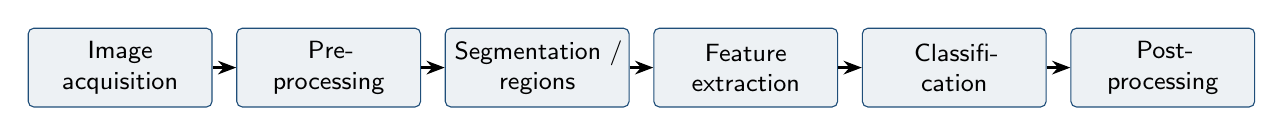
\begin{tikzpicture}[node distance=3mm,
  box/.style={draw=accent, fill=accent!8, rounded corners=2pt, align=center,
    font=\sffamily\small, minimum height=10mm, text width=21mm},
  >={Stealth}]
  \node[box] (a) {Image\\acquisition};
  \node[box, right=of a] (b) {Pre-\\processing};
  \node[box, right=of b] (c) {Segmentation /\\regions};
  \node[box, right=of c] (d) {Feature\\extraction};
  \node[box, right=of d] (e) {Classifi-\\cation};
  \node[box, right=of e] (f) {Post-\\processing};
  \foreach \s/\t in {a/b,b/c,c/d,d/e,e/f} \draw[->, thick] (\s) -- (\t);
\end{tikzpicture}}
\end{center}
\noindent
Acquisition delivers the image; preprocessing removes noise and normalizes
contrast or geometry; segmentation (or a sliding window / region proposals)
defines the units to be analyzed; feature extraction describes each unit by a
vector (color, texture, HOG, SIFT, \dots); a classifier maps features to labels;
postprocessing adds context (non-maximum suppression, MRF/CRF smoothing,
consistency checks) and produces the final interpretation. In deep networks,
feature extraction and classification are learned jointly end to end.

% =====================================================================
\topic{Classifiers and Bag of Visual Words}{Q9--Q16}

\idea{A classifier maps a feature vector $\mathbf{x}$ to a class. Linear
classifiers draw one hyperplane; MLPs stack nonlinear layers to bend the
decision boundary; random forests combine many randomized decision trees.
Bag of Visual Words is a way to turn a variable number of local features into
one fixed-length vector that any of these classifiers can take.}

\q{9}{What are typical classifiers used in image analysis tasks?}
$k$-nearest neighbors; Bayes / Naive Bayes classifiers (generative, based on
class-conditional densities); linear classifiers (perceptron, logistic
regression); support vector machines (linear or with kernels); decision trees,
random forests, and boosting (AdaBoost); neural networks (MLPs and, today
dominant, convolutional networks).

\q{10}{What is the general idea of the ``Bag of (Visual) Words'' approach?}
Borrowed from text retrieval, where a document is represented by word counts.
\begin{enumerate}
  \item Detect keypoints / sample patches and compute local descriptors (e.g.\
    SIFT) on all training images.
  \item Cluster the descriptors (e.g.\ $k$-means); each cluster center is a
    \emph{visual word}, all centers form the \emph{codebook} (vocabulary).
  \item Represent an image by the histogram of visual-word occurrences: assign
    each of its descriptors to the nearest word and count.
  \item Classify the fixed-length histogram (e.g.\ SVM, Naive Bayes).
\end{enumerate}
\noindent
The representation is robust to occlusion and object position but discards all
spatial layout (``bag''); spatial pyramids re-add coarse layout.

\q{11}{What is a linear classifier?}
A classifier whose decision depends on a linear function of the features,
\[
  g(\mathbf{x}) = \mathbf{w}^\top\mathbf{x} + b, \qquad
  \text{class} = \begin{cases} 1 & g(\mathbf{x}) > 0\\ 2 & \text{otherwise.}\end{cases}
\]
\noindent
The decision boundary $g(\mathbf{x})=0$ is a hyperplane with normal
$\mathbf{w}$ and offset $b$. Examples: perceptron, logistic regression, linear
SVM, linear discriminant analysis. It can only separate linearly separable
classes (fails on XOR), unless the features are first mapped nonlinearly.

\q{12}{What does MLP stand for?}
\emph{Multi-Layer Perceptron}.

\q{13}{What is the general principle of an MLP?}
A feed-forward network of layers of neurons. Each neuron $j$ computes a weighted
sum of its inputs plus a bias and passes it through a nonlinear activation $f$:
\[
  a_j = \sum_i w_{ji}\, z_i + b_j, \qquad z_j = f(a_j).
\]
\noindent
Input layer $\rightarrow$ one or more hidden layers $\rightarrow$ output layer,
each fully connected to the next. The hidden layers learn a nonlinear feature
transform so that the output layer can separate the classes; with one hidden
layer of sufficient size an MLP is a universal function approximator. The
weights are learned by minimizing a loss (squared error, cross-entropy) with
gradient descent, gradients obtained by backpropagation.

\q{14}{What is usually referred to as ``backprop''?}
\emph{Error backpropagation}: the efficient computation of the gradient of the
loss $E$ with respect to every weight via the chain rule. After a forward pass,
error signals $\delta$ are propagated from the output back through the network:
\[
  \delta_k = f'(a_k)\,\frac{\partial E}{\partial z_k}\ \text{(output)}, \qquad
  \delta_j = f'(a_j)\sum_k w_{kj}\,\delta_k\ \text{(hidden)}, \qquad
  \frac{\partial E}{\partial w_{ji}} = \delta_j\, z_i .
\]
\noindent
The gradients are then used in a gradient-descent update (Q109). For squared
error $E=\tfrac12(z_k-t_k)^2$ the output term is $\delta_k=f'(a_k)(z_k-t_k)$.

\q{15}{What does RF stand for?}
\emph{Random Forest}.

\q{16}{What is the general principle of an RF?}
An ensemble of $T$ decision trees. Each tree routes a sample from the root to a
leaf by binary tests on the features; the leaf stores a class distribution.
Randomness makes the trees different (decorrelated):
\begin{itemize}
  \item each tree is trained on a bootstrap sample of the training data
    (\emph{bagging});
  \item at each node only a random subset of features / candidate tests is
    evaluated, and the one with the highest information gain
    (largest entropy or Gini reduction) is chosen.
\end{itemize}
\noindent
Prediction: average the leaf distributions (or majority vote) over all trees.
Averaging many high-variance, low-bias trees reduces variance and overfitting.
Forests are fast, handle many classes naturally, and give probabilistic
outputs.

% =====================================================================
\topic{Fourier Transform}{Q17--Q23}

\idea{The Fourier transform rewrites a signal as a sum of sinusoids. Narrow in
one domain means wide in the other, convolution becomes multiplication, and a
real signal has a mirror-symmetric spectrum.}

\q{17}{What is the general principle of the Fourier transformation?}
Every (sufficiently well-behaved) signal can be written as a superposition of
complex exponentials $e^{i2\pi ux}=\cos(2\pi ux)+i\sin(2\pi ux)$ of different
frequencies $u$. The transform computes, for each frequency, how much of it is in
the signal (amplitude) and with which shift (phase):
\[
  F(u) = \int_{-\infty}^{\infty} f(x)\, e^{-i2\pi ux}\,\mathrm{d}x, \qquad
  f(x) = \int_{-\infty}^{\infty} F(u)\, e^{i2\pi ux}\,\mathrm{d}u .
\]
\noindent
It is a change of basis from the spatial to the frequency domain; no
information is lost. For images: 2D transform over $(u,v)$; for sampled data:
the DFT, computed with the FFT.

\q{18}{What is the Fourier spectrum of a sine function?}
\[
  \sin(2\pi u_0 x)\ \longleftrightarrow\
  \tfrac{i}{2}\big[\delta(u+u_0) - \delta(u-u_0)\big],
  \qquad
  \cos(2\pi u_0 x)\ \longleftrightarrow\
  \tfrac{1}{2}\big[\delta(u+u_0) + \delta(u-u_0)\big].
\]
\noindent
Two Dirac impulses at $\pm u_0$. For the sine they are purely imaginary and of
opposite sign (odd signal); the magnitude spectrum shows two spikes of height
$\tfrac12$.

\q{19}{What is the Fourier spectrum of a rectangular function?}
A sinc function. For a box of height 1 and width $a$:
\[
  \operatorname{rect}(x/a)\ \longleftrightarrow\ a\,\operatorname{sinc}(au)
  = \frac{\sin(\pi a u)}{\pi u}.
\]
\noindent
Main lobe at $u=0$ of height $a$, zeros at $u=k/a$. A wider box gives a narrower
sinc (and vice versa).

\q{20}{What is the Fourier spectrum of a sinc function?}
A rectangular function (duality of the transform pair):
$\operatorname{sinc}(x)\longleftrightarrow\operatorname{rect}(u)$. This is why
the sinc is the ideal low-pass filter kernel: its spectrum passes all
frequencies below a cutoff and nothing above.

\begin{figure}[ht]
\centering
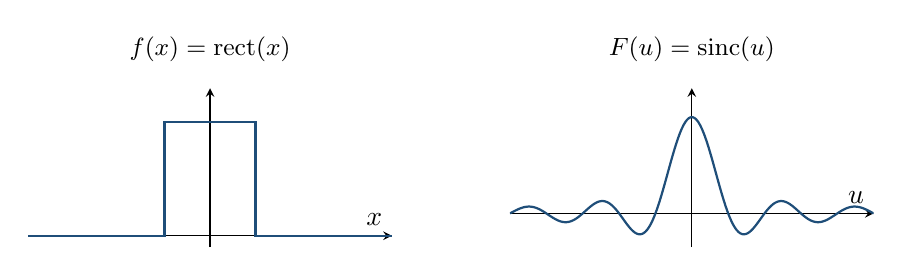
\begin{tikzpicture}
  \begin{axis}[name=l, width=6.2cm, height=3.6cm, axis lines=middle,
    xmin=-2, xmax=2, ymin=-0.1, ymax=1.3, ticks=none,
    xlabel={$x$}, title={\small $f(x)=\operatorname{rect}(x)$}]
    \addplot[accent, thick] coordinates {(-2,0) (-0.5,0) (-0.5,1) (0.5,1) (0.5,0) (2,0)};
  \end{axis}
  \begin{axis}[at={($(l.east)+(1.5cm,0)$)}, anchor=west, width=6.2cm, height=3.6cm,
    axis lines=middle, xmin=-5, xmax=5, ymin=-0.35, ymax=1.3, ticks=none,
    xlabel={$u$}, title={\small $F(u)=\operatorname{sinc}(u)$}]
    \addplot[accent, thick, samples=200, domain=-5:5]
      {abs(x)<0.001 ? 1 : sin(deg(pi*x))/(pi*x)};
  \end{axis}
\end{tikzpicture}
\caption{The rect--sinc pair. Read left to right it answers Q19, read right to
left it answers Q20.}
\end{figure}

\q{21}{What is the convolution theorem?}
Convolution in the spatial domain equals multiplication in the frequency domain,
and vice versa:
\[
  f * g \ \longleftrightarrow\ F\cdot G, \qquad
  f\cdot g \ \longleftrightarrow\ F * G .
\]
\noindent
Consequences: filtering can be done by multiplying spectra (fast for large
kernels via FFT), and a filter's effect is read off its spectrum (Gaussian
$\rightarrow$ Gaussian low-pass).

\q{22}{What is the correlation theorem?}
Cross-correlation corresponds to multiplying one spectrum with the complex
conjugate of the other:
\[
  f \star g \ \longleftrightarrow\ F^{*}\cdot G,
  \qquad \text{special case: } f\star f \ \longleftrightarrow\ |F|^2 .
\]
\noindent
The autocorrelation of a signal is the inverse transform of its power spectrum
(Wiener--Khinchin). Used for fast template matching.

\q{23}{Which property does the spectrum of a real function fulfill?}
It is Hermitian (conjugate symmetric): $F(-u) = F^{*}(u)$. Hence the magnitude
$|F(u)|$ is even, the phase is odd, the real part is even and the imaginary part
is odd. Half of the spectrum is redundant. If $f$ is additionally even, $F$ is
real and even; if $f$ is real and odd, $F$ is imaginary and odd (as for the sine
in Q18).

% =====================================================================
\topic{Fourier Descriptors}{Q24--Q29}

\idea{Walk around an object's contour, write each boundary point as a complex
number $z_k = x_k + i\,y_k$, and take the DFT. Low frequencies describe coarse
shape, high frequencies fine detail. Translation, scale, rotation and start
point each affect the coefficients in a simple way, so they can be normalized
away.}

\q{24}{How to extract a normalized Fourier descriptor given a grayscale image?}
\begin{enumerate}
  \item Segment the object (e.g.\ thresholding) to a binary image.
  \item Trace the outer contour (boundary following) and sample $N$ points,
    ideally equidistant along the contour.
  \item Write the points as complex numbers $z_k = x_k + i\,y_k$,
    $k=0,\dots,N-1$.
  \item Compute the DFT $Z_n = \sum_{k} z_k\, e^{-i2\pi nk/N}$.
  \item Normalize: set $Z_0=0$ (translation), divide all coefficients by
    $|Z_1|$ (scale), keep only magnitudes $|Z_n|$ (rotation and start point).
  \item Optionally keep only the first few low-frequency coefficients as a
    compact feature vector.
\end{enumerate}

\q{25}{How does the Fourier descriptor change when the object is translated?}
Only $Z_0$ changes; it is the (scaled) centroid of the contour. A shift
$z_k\mapsto z_k+\Delta$ adds $N\Delta$ to $Z_0$ and leaves every $Z_n$,
$n\neq 0$, unchanged. Normalization: drop $Z_0$.

\q{26}{How does the Fourier descriptor change when the object is scaled?}
All coefficients are multiplied by the scale factor $s$: $Z_n\mapsto s\,Z_n$
(linearity). Normalization: divide by $|Z_1|$ (or another reference
coefficient).

\q{27}{How does the Fourier descriptor change when the object is rotated?}
Rotation by $\varphi$ multiplies each point by $e^{i\varphi}$, hence every
coefficient: $Z_n\mapsto e^{i\varphi}Z_n$. Magnitudes stay unchanged, only
phases shift. A different start point $k_0$ gives
$Z_n\mapsto e^{i2\pi n k_0/N}Z_n$, again a pure phase change. Using $|Z_n|$
removes both.

\begin{table}[ht]
  \centering\small
  \begin{tabular}{@{}lll@{}}
    \toprule
    Transformation & Effect on coefficients & Normalization \\
    \midrule
    Translation by $\Delta$ & $Z_0 \mapsto Z_0 + N\Delta$, rest unchanged & set $Z_0=0$ \\
    Scaling by $s$ & $Z_n \mapsto s\,Z_n$ & divide by $|Z_1|$ \\
    Rotation by $\varphi$ & $Z_n \mapsto e^{i\varphi} Z_n$ & use $|Z_n|$ \\
    Start point shift $k_0$ & $Z_n \mapsto e^{i2\pi nk_0/N} Z_n$ & use $|Z_n|$ \\
    \bottomrule
  \end{tabular}
  \caption{How Fourier descriptors react to similarity transforms and how each
  effect is removed.}
\end{table}

\q{28}{How to smooth a shape using the framework of Fourier descriptors?}
Low-pass filter the descriptor: keep the low-frequency coefficients
$Z_n$ for $|n|\le M$ (with the DFT indexing, the first and the last $M$
coefficients), set the others to zero, and apply the inverse DFT. The
reconstructed contour keeps the overall shape and loses fine wiggles and noise.
Fewer kept coefficients means a smoother shape (with only $Z_0,Z_1$: a circle).

\q{29}{What are disadvantages of Fourier descriptors, i.e.\ when will they fail?}
\begin{itemize}
  \item They need a correct segmentation and a single closed contour; broken
    contours, merged objects, or noise at the boundary spoil them.
  \item Occlusion fails: a missing part changes all coefficients, since each
    coefficient is global.
  \item Only the outer contour is described; holes and inner structure,
    texture, and color are ignored; objects of several parts are hard.
  \item Magnitude-only descriptors discard phase, so different shapes can have
    the same descriptor.
  \item Invariance only to similarity transforms, not to perspective/affine
    distortion or articulation (different views of a 3D object).
\end{itemize}

% =====================================================================
\topic{Saliency and Scale Space}{Q30--Q38}

\idea{Saliency asks \emph{where} an image is worth looking at. The classical
computational answer (Kadir/Brady) says: where the local intensity distribution
is complex (high entropy) \emph{and} this complexity is tied to a distinct
scale. Evaluating ``scale'' needs a multi-scale representation: an image
pyramid or a Gaussian scale space.}

\q{30}{Is biological saliency a pure bottom-up, a pure top-down process, or a
mixture of both?}
A mixture. Bottom-up, stimulus-driven factors (contrast, color, motion, an odd
item among uniform ones) attract attention automatically; top-down factors
(the current task, knowledge, expectations) modulate where we look. The same
scene is scanned differently when searching for different things.

\q{31}{What is the aim of saliency operators for image analysis?}
To find regions that stand out from their surroundings, i.e.\ are rare,
informative, and distinctive, and to restrict further (expensive) processing to
them. In object models they supply repeatable interest points / regions at
which descriptors are computed and matched.

\q{32}{Describe a computational model of saliency.}
Kadir/Brady scale saliency. For each position $\mathbf{x}$ and a range of
window sizes $s$, compute the histogram $p(I,s,\mathbf{x})$ of intensities
inside the window and its entropy
\[
  H_D(s,\mathbf{x}) = -\sum_I p(I,s,\mathbf{x})\log_2 p(I,s,\mathbf{x}).
\]
\noindent
Keep the scales $s_p$ where $H_D$ has a peak over $s$. Weight each peak by how
strongly the distribution changes across scale,
$W_D(s,\mathbf{x}) = s\sum_I |\partial p(I,s,\mathbf{x})/\partial s|$.
Saliency is $y(s_p,\mathbf{x}) = H_D(s_p,\mathbf{x})\,W_D(s_p,\mathbf{x})$.
The most salient (position, scale) pairs are selected. Noise and regular
textures have high but flat entropy over scale, so they are not salient; a blob
has an entropy peak where the window just encloses it.

An alternative, biologically inspired model is Itti/Koch: intensity, color and
orientation channels on a Gaussian pyramid, center--surround differences,
normalization, summation into one saliency map, winner-take-all with
inhibition of return.

\q{33}{What is the entropy of a signal?}
The average information content, i.e.\ the uncertainty of the value
distribution:
\[
  H = -\sum_i p_i \log_2 p_i \quad [\text{bit}].
\]
\noindent
$H=0$ if one value occurs with certainty; $H$ is maximal ($\log_2 K$) for a
uniform distribution over $K$ values. For images, $p_i$ is the normalized
gray-value histogram.

\q{34}{Does a textured image have a higher or lower entropy than a homogeneous
image?}
Higher. A homogeneous image has one gray value, $p=1$, so $H=0$. A textured
image spreads over many gray values, the histogram is flatter, so $H$ is larger.
Note: histogram entropy ignores spatial arrangement; shuffling the pixels does
not change it.

\q{35}{What is an image pyramid?}
A stack of copies of the image at decreasing resolution. Each level is obtained
by low-pass filtering (Gaussian) and subsampling the previous level, typically
by a factor of 2 in each direction ($R_0, R_{-1}, R_{-2},\dots$). The total
memory is at most $\tfrac43$ of the original. Used for coarse-to-fine search
and multi-scale detection (e.g.\ HOG/DPM feature pyramids). The Laplacian
pyramid stores the differences between levels.

\q{36}{What is a linear Gaussian scale space?}
A one-parameter family of images obtained by convolving the original with
Gaussians of increasing width $t$, \emph{without} subsampling:
\[
  L(\mathbf{x},t) = L(\mathbf{x}) * G(\mathbf{x},t), \qquad
  G(\mathbf{x},t) = (\pi t)^{-n/2}\exp\!\left(-\frac{|\mathbf{x}|^2}{t}\right).
\]
\noindent
All levels keep the full resolution; fine structures disappear as $t$ grows.
The Gaussian is the unique kernel for which coarser scales create no new
structures (causality), and the family satisfies the diffusion (heat) equation.
Difference to the pyramid: continuous scale, constant resolution, more memory.

\q{37}{What is the modern approach to image saliency?}
Learning saliency from data with deep (convolutional) neural networks, trained
on large datasets of human eye fixations or annotated salient objects, instead
of hand-crafted information-theoretic measures. Trade-off: better predictions
and task adaptation, but a need for much labeled data.

\q{38}{What are possible applications of saliency operators for images?}
Interest point / region detection for matching, registration, and part-based
object models (e.g.\ ISM); focus of attention and computation (detection
candidates, robot vision); image compression (more bits for salient regions);
thumbnailing, cropping, and content-aware retargeting; evaluating advertising
and design; video surveillance.

% =====================================================================
\topic{Hough Transform}{Q39--Q46}

\idea{Detect shapes by \emph{voting}: each piece of image evidence votes for all
shape parameters consistent with it; parameters that many pieces agree on appear
as peaks in the accumulator. The accumulator has one dimension per unknown
parameter.}

\q{39}{State a parametric model of a line.}
Slope--intercept form $y = mx + c$ (fails for vertical lines, $m$ unbounded)
or, preferred for Hough, the Hesse normal form
\[
  x\cos\theta + y\sin\theta = r,
\]
\noindent
with $\theta$ the angle of the line normal and $r$ the distance of the line from
the origin. Both parameters are bounded.

\q{40}{How is a point on a line in image space represented in the parameter
space, if the line detector is based on the Radon transformation?}
As a \emph{sinusoid}. A single point $(x_0,y_0)$ lies on infinitely many lines;
sweeping $\theta$ gives $r(\theta) = x_0\cos\theta + y_0\sin\theta$. The point
votes for every cell on this curve. All points of one line produce sinusoids
that intersect in one common point $(r,\theta)$: the parameters of that line.

\q{41}{How is a point on a line in image space represented in the parameter
space, if the Hough line detector is used?}
As a \emph{single point}. The gradient-based Hough detector uses edge pixels
with their gradient direction. The gradient fixes $\theta$, and $r$ follows from
$r = x_0\cos\theta + y_0\sin\theta$, so each edge pixel votes for exactly one
cell $(r,\theta)$.

\begin{figure}[ht]
\centering
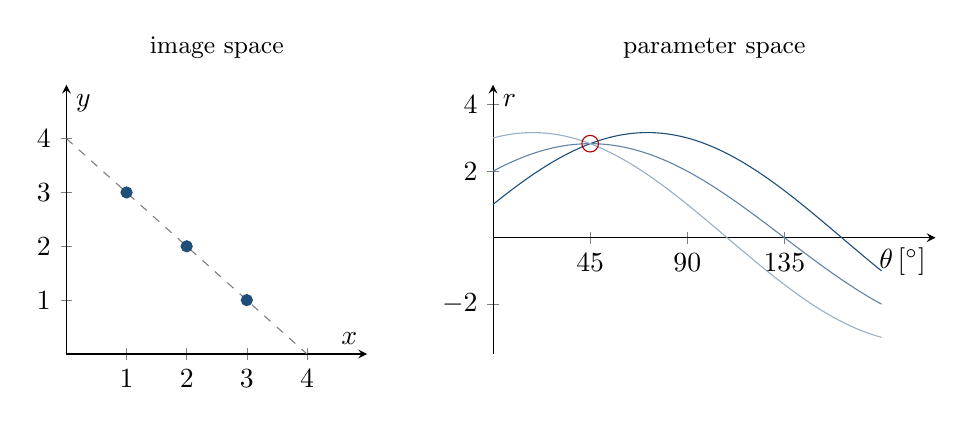
\begin{tikzpicture}
  \begin{axis}[name=img, width=5.4cm, height=5.0cm, axis lines=middle,
    xmin=0, xmax=5, ymin=0, ymax=5, xtick={1,2,3,4}, ytick={1,2,3,4},
    xlabel={$x$}, ylabel={$y$}, title={\small image space}]
    \addplot[gray, dashed, domain=0:4] {4-x};
    \addplot[only marks, mark=*, accent] coordinates {(1,3) (2,2) (3,1)};
  \end{axis}
  \begin{axis}[at={($(img.east)+(1.6cm,0)$)}, anchor=west, width=7.2cm,
    height=5.0cm, axis lines=middle, xmin=0, xmax=205, ymin=-3.5, ymax=4.6,
    xtick={45,90,135}, ytick={-2,2,4},
    xlabel={$\theta\,[^\circ]$}, ylabel={$r$}, title={\small parameter space},
    every axis x label/.style={at={(current axis.right of origin)}, anchor=north east}]
    \addplot[accent, domain=0:180, samples=90] {cos(x)+3*sin(x)};
    \addplot[accent!70, domain=0:180, samples=90] {2*cos(x)+2*sin(x)};
    \addplot[accent!45, domain=0:180, samples=90] {3*cos(x)+sin(x)};
    \addplot[only marks, mark=o, mark size=3pt, red!70!black] coordinates {(45,2.828)};
  \end{axis}
\end{tikzpicture}
\caption{Radon view: the three collinear points on $x+y=4$ trace three sinusoids
that meet in one cell, $\theta=45^\circ$, $r=4/\sqrt2\approx2.83$ (circle). With
gradient information (Hough), each point would vote only for that circled cell.}
\end{figure}

\q{42}{What is the working principle of the Hough line detector?}
\begin{enumerate}
  \item Detect edge pixels (e.g.\ gradient magnitude above a threshold) and
    their gradient direction.
  \item Discretize the parameter space $(r,\theta)$ into an accumulator
    $H(r,\theta)$, initialized to zero.
  \item Each edge pixel votes: $\theta$ from the gradient direction,
    $r = x\cos\theta + y\sin\theta$, $H(r,\theta) \mathrel{+}= 1$ (or
    $+=$ gradient magnitude). Without gradients: vote along the full sinusoid.
  \item Find local maxima in $H$ above a threshold
    (non-maximum suppression); each peak is a detected line.
\end{enumerate}
\noindent
Robust to noise, gaps and occlusion, since missing points only lower a peak.

\q{43}{What is the relationship between the gradient of a line and the
orientation of the line?}
The image gradient at an edge is \emph{perpendicular} to the line. Its
direction $\theta = \operatorname{atan2}(g_y, g_x)$ is exactly the normal angle
$\theta$ of the Hesse form; the line itself runs at $\theta \pm 90^\circ$.
In slope form, the line slope is $m = -\cot\theta = -1/\tan\theta$.

\q{44}{How many dimensions has a Hough circle detector?}
Three: center $(x_c, y_c)$ and radius $\rho$, from
$(x-x_c)^2 + (y-y_c)^2 = \rho^2$. With known radius: two. Gradient direction
reduces the votes per pixel: for each $\rho$ the center lies at distance $\rho$
along the gradient direction.

\q{45}{What is the R-table?}
The lookup table of the Generalized Hough Transform describing an arbitrary
template shape. Choose a reference point $\mathbf{a}$ (e.g.\ the centroid). For
every boundary point $\mathbf{x}$ of the template, compute the gradient
orientation $\phi$ and the displacement $\mathbf{r} = \mathbf{a}-\mathbf{x}$.
The table is indexed by quantized $\phi$; row $\phi$ lists all displacement
vectors of boundary points with that orientation. At detection, each edge pixel
looks up its $\phi$ and votes for $\mathbf{x}+\mathbf{r}$ for every stored
$\mathbf{r}$.

\q{46}{How many dimensions has the voting space of the Generalized Hough
Transform?}
Two ($x$, $y$ of the reference point) if only translation is unknown. With
unknown scale $s$ and rotation $\theta$: four, $(x,y,s,\theta)$ (the stored
vectors are scaled and rotated before voting).

% =====================================================================
\topic{Part-Based Object Detection}{Q47--Q58}

\idea{Instead of one rigid template, objects are modeled as a set of local parts
with a spatial layout. ISM and Hough forests let parts \emph{vote} for the
object center (a learned, probabilistic Generalized Hough Transform). HOG
describes a window by local gradient histograms; DPM adds deformable parts on
top of HOG.}

\q{47}{What does ISM stand for?}
\emph{Implicit Shape Model} (Leibe, Leonardis, Schiele).

\q{48}{What are the differences between the Generalized Hough Transform and the
ISM?}
\begin{table}[ht]
  \centering\small
  \begin{tabularx}{\linewidth}{@{}l>{\raggedright\arraybackslash}X>{\raggedright\arraybackslash}X@{}}
    \toprule
    & Generalized Hough Transform & Implicit Shape Model \\
    \midrule
    Evidence & edge pixels & local appearance patches at interest points \\
    Index & gradient orientation (R-table row) & codebook entry (visual word) \\
    Model source & one hand-given template shape & learned from many training images \\
    Scope & specific rigid shape & object category, intra-class variation \\
    Votes & deterministic, equal weight & probabilistic, weighted; soft matching to several entries \\
    Vote space & discrete accumulator & continuous $(x,y,s)$, modes via mean shift \\
    Extras & --- & back-projection for verification and top-down segmentation \\
    \bottomrule
  \end{tabularx}
  \caption{GHT versus ISM. The ISM keeps the voting idea but replaces the R-table
  by a learned codebook with occurrence distributions.}
\end{table}

\q{49}{What is the algorithm to train the ISM?}
\begin{enumerate}
  \item Training images of the category with known object center and scale
    (bounding box, optionally figure--ground masks).
  \item Detect interest points (e.g.\ Harris--Laplace, DoG, or salient regions)
    and extract patches / descriptors.
  \item Cluster all descriptors (agglomerative clustering) into a codebook of
    visual words.
  \item Match every training patch again to the codebook (all entries with
    similarity above a threshold $t$) and record, for each matching entry, the
    \emph{occurrence}: relative position to the object center, scale, and
    optionally the local figure--ground mask.
\end{enumerate}

\q{50}{What is the algorithm to apply the ISM?}
\begin{enumerate}
  \item Detect interest points in the test image and extract descriptors.
  \item Match each descriptor to all codebook entries with similarity $> t$.
  \item Each matched entry casts votes for object center and scale
    $(x,y,s)$ using its stored occurrences, with weight
    $\frac{1}{|\text{matched entries}|}\cdot\frac{1}{|\text{occurrences}|}$.
  \item Find maxima in the continuous voting space with mean-shift mode
    search; each mode is an object hypothesis.
  \item Back-project the votes that support a hypothesis to verify it and to
    obtain a top-down segmentation.
\end{enumerate}

\q{51}{What is a Hough Forest?}
A random forest that performs Hough voting (Gall, Lempitsky). Trained on
image patches from object and background; each leaf stores a class probability
and the offset vectors from positive patches to the object center. At test time
dense patches are passed through all trees, each reached leaf casts weighted
votes for the object center, the votes are accumulated in a Hough image, and
peaks are detections. It is a discriminatively trained codebook replacing the
clustering step of the ISM.

\q{52}{What kind of node tests are used in a Hough Forest?}
Simple binary pixel comparisons on a feature channel $I^a$ (e.g.\ intensity,
gradients, HOG-like channels, Lab color):
\[
  t(\mathcal{P}) = \begin{cases}
    0 & I^a(\mathbf{p}) < I^a(\mathbf{q}) + \tau\\ 1 & \text{otherwise,}
  \end{cases}
\]
\noindent
with random channel $a$, positions $\mathbf{p},\mathbf{q}$ in the patch, and
threshold $\tau$. Many random candidates are generated; the best by the
energy criterion (Q53) is kept.

\q{53}{What kind of energy functions are used in a Hough Forest?}
Two uncertainty measures, one chosen at random per node:
\begin{itemize}
  \item \emph{Class-label uncertainty}: entropy of the class labels in the
    child sets, $|A|\,H(A)$ summed over children (maximizing information gain).
  \item \emph{Offset uncertainty}: spread of the offset vectors of the positive
    patches, $\sum_{i}\|\mathbf{d}_i - \bar{\mathbf{d}}\|^2$ per child.
\end{itemize}
\noindent
The split minimizing the chosen energy is taken. Thus leaves become both pure in
class and consistent in the vote they cast.

\q{54}{Which information is stored in the leafs of a Hough Forest?}
The proportion $C_L$ of object (foreground) patches that reached the leaf,
i.e.\ the class probability, and the list $D_L = \{\mathbf{d}_i\}$ of offset
vectors from these object patches to the object center. At test time each
offset is a vote with weight $C_L/|D_L|$.

\q{55}{What does HOG stand for?}
\emph{Histograms of Oriented Gradients} (Dalal, Triggs).

\q{56}{How is a HOG descriptor computed given an image?}
\begin{enumerate}
  \item (Optional) gamma / color normalization.
  \item Gradients with the simple filters $[-1,0,1]$ and $[-1,0,1]^\top$;
    magnitude and orientation per pixel.
  \item Divide the detection window (e.g.\ $64\times128$) into cells of
    $8\times8$ pixels. Per cell, build a histogram of 9 orientation bins over
    $0^\circ$--$180^\circ$; each pixel votes with its gradient magnitude
    (interpolated between neighboring bins).
  \item Group $2\times2$ cells into overlapping blocks (stride one cell) and
    normalize each block vector (L2-Hys) for illumination invariance.
  \item Concatenate all normalized block vectors ($7\times15$ blocks
    $\times\,36 = 3780$ dimensions for $64\times128$).
\end{enumerate}
\noindent
Classification: linear SVM, applied with a sliding window over an image
pyramid.

\q{57}{What does DPM stand for?}
\emph{Deformable Part Model} (Felzenszwalb et al.).

\q{58}{What is the general working principle of a DPM?}
An object is a coarse \emph{root filter} (HOG template of the whole object)
plus several \emph{part filters} at twice the resolution, each with an anchor
position and a quadratic deformation cost. The score of a hypothesis at root
position $p_0$ is
\[
  \text{score}(p_0) = F_0\cdot\phi(p_0)
  + \sum_{i=1}^{n}\max_{p_i}\big[F_i\cdot\phi(p_i) - d_i\cdot\phi_d(\Delta p_i)\big]
  + b ,
\]
\noindent
i.e.\ each part is placed where its appearance score minus deformation penalty
is best. Evaluated with a sliding window over a HOG pyramid; the max over part
positions is computed efficiently with generalized distance transforms. Several
components (mixture) cover different viewpoints. Training: latent SVM, since
part positions are not annotated, with hard-negative mining.

% =====================================================================
\topic{Probability and Bayesian Decisions}{Q59--Q76}

\idea{All rules follow from two identities: the product rule
$P(A,B)=P(A\mid B)P(B)$ and the sum rule $P(A)=\sum_B P(A,B)$. Bayes' theorem
combines them. Classification then means picking the class with the best
posterior (MAP), likelihood (ML), or lowest expected cost.}

\q{59}{Which properties need a function to fulfill to be a probability?}
Kolmogorov axioms, for events of a sample space $\Omega$:
(1) $P(A)\ge 0$; (2) $P(\Omega)=1$; (3) additivity: for disjoint events
$P(A\cup B)=P(A)+P(B)$ (countable additivity in general). Consequences:
$0\le P(A)\le 1$, $P(\bar A)=1-P(A)$, $P(\emptyset)=0$.

\q{60}{What are the differences between a probability and a probability
density?}
\begin{table}[ht]
  \centering\small
  \begin{tabular}{@{}lll@{}}
    \toprule
    & Probability $P$ & Density $p$ \\
    \midrule
    Variable & discrete events & continuous variable \\
    Range & $0\le P\le 1$ & $p\ge 0$, may exceed 1 \\
    Normalization & $\sum_x P(x)=1$ & $\int p(x)\,\mathrm{d}x=1$ \\
    Meaning of value & probability of the event & probability per unit ($x$) \\
    Single value & $P(x)$ can be $>0$ & $P(X=x)=0$; only intervals: $\int_a^b p\,\mathrm{d}x$ \\
    \bottomrule
  \end{tabular}
  \caption{Probability versus probability density.}
\end{table}

\q{61}{What is the joint probability of two events?}
$P(A,B) = P(A\cap B)$: the probability that $A$ \emph{and} $B$ occur together.

\q{62}{What is the conditional probability of an event A given B?}
The probability of $A$ when $B$ is known to have occurred:
$P(A\mid B) = \dfrac{P(A,B)}{P(B)}$, defined for $P(B)>0$.

\q{63}{What is marginalization?}
Removing a variable from a joint distribution by summing (or integrating) over
all its values (sum rule):
$P(A) = \sum_B P(A,B) = \sum_B P(A\mid B)P(B)$, respectively
$p(x)=\int p(x,y)\,\mathrm{d}y$.

\q{64}{How can the joint probability of two events be factorized into
probabilities of the individual events?}
Product rule: $P(A,B) = P(A\mid B)\,P(B) = P(B\mid A)\,P(A)$. For many
variables (chain rule):
$P(x_1,\dots,x_n) = \prod_i P(x_i\mid x_1,\dots,x_{i-1})$.

\q{65}{If two events are independent, what is then known about their
conditional and joint probabilities?}
$P(A\mid B) = P(A)$, $P(B\mid A)=P(B)$, and $P(A,B) = P(A)\,P(B)$.

\q{66}{What is Bayes' Theorem?}
\[
  P(A\mid B) = \frac{P(B\mid A)\,P(A)}{P(B)}, \qquad
  P(B) = \sum_{A'} P(B\mid A')\,P(A').
\]
\noindent
It turns the probability of the data given a hypothesis into the probability of
the hypothesis given the data.

\q{67}{What are the technical names of all terms in Bayes' theorem?}
With class $c$ and observation $x$:
$\underbrace{P(c\mid x)}_{\text{posterior}} =
\dfrac{\overbrace{P(x\mid c)}^{\text{likelihood}}\ \overbrace{P(c)}^{\text{prior}}}
{\underbrace{P(x)}_{\text{evidence}}}$.
The evidence is also called marginal likelihood or normalization constant.

\q{68}{Given the joint probability of two events, derive Bayes' theorem.}
Factorize the joint in both orders (product rule):
$P(A,B) = P(A\mid B)P(B)$ and $P(A,B)=P(B\mid A)P(A)$. Equate the right-hand
sides, $P(A\mid B)P(B) = P(B\mid A)P(A)$, and divide by $P(B)>0$:
$P(A\mid B) = P(B\mid A)P(A)/P(B)$. The denominator follows by
marginalization: $P(B)=\sum_A P(B\mid A)P(A)$.

\q{69}{What does MAP stand for?}
\emph{Maximum A Posteriori}.

\q{70}{What is the decision rule of a MAP estimator?}
Choose the class with the highest posterior:
\[
  \hat c = \arg\max_c P(c\mid x) = \arg\max_c P(x\mid c)\,P(c).
\]
\noindent
The evidence $P(x)$ is the same for all classes and can be dropped. MAP
minimizes the probability of error (Bayes classifier).

\q{71}{What does ML stand for (in the context of probability theory)?}
\emph{Maximum Likelihood}.

\q{72}{What is the decision rule of a ML estimator?}
Choose the class under which the observation is most likely, ignoring priors:
$\hat c = \arg\max_c P(x\mid c)$.

\q{73}{In which case are ML and MAP equivalent?}
When the prior is uniform, $P(c)=\text{const}$ for all classes; it then does
not change the $\arg\max$. (For parameter estimation: flat prior over
parameters.)

\q{74}{What is Naive Bayes?}
A Bayes classifier with the ``naive'' assumption that the features are
conditionally independent given the class:
\[
  P(\mathbf{x}\mid c) = \prod_{i=1}^{D} P(x_i\mid c), \qquad
  \hat c = \arg\max_c P(c)\prod_i P(x_i\mid c).
\]
\noindent
Instead of one $D$-dimensional density per class, only $D$ one-dimensional
densities are estimated, which beats the curse of dimensionality. It often works
well even though the assumption rarely holds exactly. Zero counts are avoided by
the Laplace correction (Q81).

\q{75}{How is it possible to take the cost of a decision into account?}
Define a loss $\lambda(\alpha_i\mid c_j)$: the cost of action (decision)
$\alpha_i$ when the true class is $c_j$. The conditional risk of an action is
the expected loss under the posterior,
\[
  R(\alpha_i\mid x) = \sum_j \lambda(\alpha_i\mid c_j)\,P(c_j\mid x),
\]
\noindent
and the Bayes decision rule picks the action with minimum risk. With 0/1 loss
this reduces to MAP. Asymmetric costs shift the boundary (e.g.\ missing a tumor
costs more than a false alarm); a ``reject'' action with fixed cost is also
possible.

\q{76}{What is a discriminant function?}
One function $g_i(\mathbf{x})$ per class; $\mathbf{x}$ is assigned to the class
with the largest value, $\hat c = \arg\max_i g_i(\mathbf{x})$. Decision
boundaries lie where $g_i = g_j$. Choices: $g_i = P(c_i\mid\mathbf{x})$,
$g_i = \ln p(\mathbf{x}\mid c_i) + \ln P(c_i)$, or $g_i=-R(\alpha_i\mid
\mathbf{x})$; any monotonically increasing transformation gives the same
decisions. For two classes a single $g = g_1 - g_2$ and its sign suffice;
linear $g$ gives a linear classifier (Q11).

% =====================================================================
\topic{Density Estimation}{Q77--Q88}

\idea{Bayes classifiers need $p(\mathbf{x}\mid c)$, which must be estimated from
samples. Either assume a model and fit its parameters (parametric) or let the
data speak directly (nonparametric). All nonparametric estimators use
$p(\mathbf{x}) \approx \frac{K}{NV}$ with $K$ of $N$ samples in a volume $V$
around $\mathbf{x}$: Parzen fixes $V$, $k$-NN fixes $K$.}

\q{77}{What is the difference between parametric and nonparametric methods of
probability estimation?}
Parametric: assume a functional form $p(\mathbf{x}\mid\boldsymbol\theta)$ (e.g.\
Gaussian) with a fixed number of parameters and estimate $\boldsymbol\theta$
from data. Compact and data-efficient, but biased if the assumed form is wrong.
Nonparametric: no fixed form; the density is built directly from the samples.
Flexible (any shape, multimodal), but needs many samples, stores the data, and
suffers from the curse of dimensionality; model complexity grows with $N$.

\q{78}{What are examples for nonparametric approaches?}
Histograms, Parzen windows / kernel density estimation, $k$-nearest neighbors.

\q{79}{What are examples for parametric approaches?}
Gaussian (normal) distribution estimated by ML or Bayesian estimation;
Bernoulli / binomial / multinomial models; exponential distribution; mixtures of
Gaussians fitted by EM (semi-parametric).

\q{80}{What is the curse of dimensionality?}
The volume of the feature space grows exponentially with the dimension $D$.
A histogram with $M$ bins per axis has $M^D$ cells, so the number of samples
needed to fill them grows exponentially; with a fixed dataset almost all cells
are empty, data become sparse, and distances between points become similar.
Nonparametric estimators (and many classifiers) therefore break down in high
dimensions unless the dimension is reduced or independence is assumed (Naive
Bayes).

\q{81}{What is the Laplace correction?}
Additive smoothing of count-based probability estimates: add one pseudo-count
to every value,
\[
  P(x=v) = \frac{n_v + 1}{N + K},
\]
\noindent
with $n_v$ the count of value $v$, $N$ samples and $K$ possible values. It
prevents zero probabilities for values unseen in training, which would otherwise
set the whole Naive Bayes product to zero.

\q{82}{What is ``Parzen Windows''?}
A nonparametric density estimation method (kernel density estimation): the
density at $\mathbf{x}$ is estimated from the samples inside a window (kernel)
of fixed size $h$ centered at $\mathbf{x}$.

\q{83}{How does Parzen Windows estimate a probability density?}
Fix the volume $V = h^D$ and count the $K$ samples inside:
$p(\mathbf{x}) \approx \frac{K}{NV}$. Written with a kernel $k$,
\[
  p(\mathbf{x}) = \frac{1}{N}\sum_{n=1}^N \frac{1}{h^D}\,
  k\!\left(\frac{\mathbf{x}-\mathbf{x}_n}{h}\right),
\]
\noindent
with a hypercube kernel (count) or, smoother, a Gaussian kernel. Every sample
places a small bump; the estimate is their average. The bandwidth $h$ controls
smoothing: small $h$ is spiky (overfitting), large $h$ oversmooths.

\q{84}{How does k-Nearest Neighbors estimate a probability density?}
Fix $K$ and let the volume adapt: grow a sphere around $\mathbf{x}$ until it
contains $K$ samples; its volume $V(\mathbf{x})$ gives
$p(\mathbf{x}) \approx \frac{K}{N\,V(\mathbf{x})}$. Dense regions give small
volumes, sparse regions large ones. The result is not a proper density (does
not integrate to 1), but for classification it yields
$P(c\mid\mathbf{x}) = K_c/K$: majority vote among the $K$ neighbors.

\q{85}{How can a Maximum-likelihood estimator be used to estimate a probability
density?}
Choose a parametric model $p(\mathbf{x}\mid\boldsymbol\theta)$ and select the
parameters under which the observed i.i.d.\ samples are most probable:
\[
  \hat{\boldsymbol\theta}_{ML} = \arg\max_{\boldsymbol\theta}
  \prod_{n=1}^N p(\mathbf{x}_n\mid\boldsymbol\theta)
  = \arg\max_{\boldsymbol\theta} \sum_{n=1}^N \ln p(\mathbf{x}_n\mid\boldsymbol\theta).
\]
\noindent
The logarithm does not change the maximizer and turns the product into a sum.
Set the gradient to zero and solve; the density estimate is then
$p(\mathbf{x}\mid\hat{\boldsymbol\theta}_{ML})$.

\q{86}{What is the ML estimate of the parameters of a Gaussian distribution?}
Sample mean and sample covariance (with $1/N$):
\[
  \hat{\boldsymbol\mu} = \frac1N\sum_{n=1}^N \mathbf{x}_n, \qquad
  \hat{\boldsymbol\Sigma} = \frac1N\sum_{n=1}^N (\mathbf{x}_n-\hat{\boldsymbol\mu})
  (\mathbf{x}_n-\hat{\boldsymbol\mu})^\top .
\]
\noindent
In 1D: $\hat\sigma^2 = \frac1N\sum(x_n-\hat\mu)^2$. This variance estimate is
biased; the unbiased one divides by $N-1$.

\q{87}{What is the basic difference between a ML estimator and a Bayesian
estimation of probability density?}
ML treats the parameters $\boldsymbol\theta$ as fixed but unknown and returns a
single point estimate $\hat{\boldsymbol\theta}$. Bayesian estimation treats
$\boldsymbol\theta$ as a random variable with a prior $p(\boldsymbol\theta)$,
computes the posterior
$p(\boldsymbol\theta\mid D)\propto p(D\mid\boldsymbol\theta)\,p(\boldsymbol\theta)$,
and averages over all parameters:
\[
  p(\mathbf{x}\mid D) = \int p(\mathbf{x}\mid\boldsymbol\theta)\,
  p(\boldsymbol\theta\mid D)\,\mathrm{d}\boldsymbol\theta .
\]
\noindent
It includes prior knowledge and the uncertainty about the parameters.

\q{88}{In which case will the ML estimator and the Bayesian estimation lead to
the same results?}
When the posterior $p(\boldsymbol\theta\mid D)$ is sharply peaked at
$\hat{\boldsymbol\theta}_{ML}$ (approximately a delta function). Then the
integral in Q87 reduces to $p(\mathbf{x}\mid\hat{\boldsymbol\theta}_{ML})$.
This happens for a large number of samples $N\to\infty$ (the likelihood
dominates) when the prior is not zero at the true value, and in particular for a
flat (uniform) prior, which makes the posterior mode equal to the ML estimate.

% =====================================================================
\topic{Graphical Models}{Q89--Q104}

\idea{A graphical model draws a joint distribution as a graph: nodes are random
variables, missing edges are conditional independencies. Directed graphs
(Bayesian networks) factorize into conditionals; undirected graphs (MRFs)
factorize into clique potentials, equivalently a sum of energies. In images,
an MRF on the pixel grid combines a data term per pixel with a smoothness term
between neighbors.}

\q{89}{What are graphical models?}
Probabilistic models whose joint distribution is represented by a graph. Nodes
are random variables; edges express direct probabilistic dependencies; the
absence of edges encodes conditional independence and thus a factorization of the
joint into local factors. Types: directed (Bayesian networks), undirected
(Markov / conditional random fields), factor graphs.

\q{90}{What are typical tasks solved with graphical models?}
Inference: computing marginals $p(x_i\mid\text{evidence})$ or the most probable
joint labeling (MAP), plus learning parameters and structure. In image
analysis: labeling problems with context such as denoising and restoration,
(semantic) segmentation, stereo matching, optical flow, and classification of
image regions with neighborhood dependencies.

\q{91}{What is conditional independence?}
$A$ and $B$ are conditionally independent given $C$, written
$A \perp B \mid C$, if
\[
  P(A,B\mid C) = P(A\mid C)\,P(B\mid C)
  \quad\Leftrightarrow\quad P(A\mid B,C) = P(A\mid C).
\]
\noindent
Once $C$ is known, $B$ gives no further information about $A$. Example: two
symptoms are dependent, but independent given the disease.

\q{92}{How to derive a graphical model given a factorization of the joint
probability?}
Directed: create one node per variable; for each factor $p(x_i\mid
\text{pa}_i)$ draw an arrow from every conditioning variable in $\text{pa}_i$ to
$x_i$. Undirected: for each potential $\psi_C(\mathbf{x}_C)$ connect all
variables in $C$ pairwise, so $C$ becomes a clique.

\q{93}{How to derive a factorization of the joint probability given a graphical
model?}
Directed: one factor per node, conditioned on its parents:
$p(\mathbf{x}) = \prod_i p(x_i\mid\text{pa}_i)$. Undirected: one potential per
maximal clique, normalized: $p(\mathbf{x}) = \frac1Z\prod_C \psi_C(\mathbf{x}_C)$.

\begin{figure}[ht]
\centering
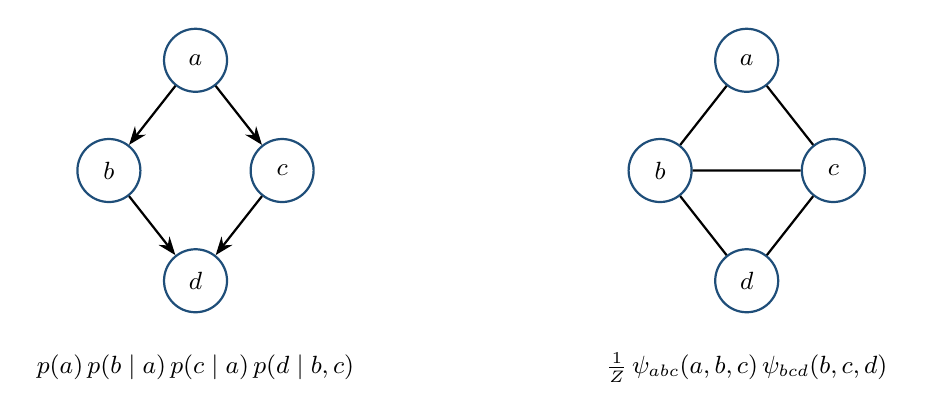
\begin{tikzpicture}[>={Stealth}, v/.style={circle, draw=accent, thick,
  minimum size=8mm, font=\small}]
  \node[v] (a) at (0,0) {$a$};
  \node[v] (b) at (-1.1,-1.4) {$b$};
  \node[v] (c) at (1.1,-1.4) {$c$};
  \node[v] (d) at (0,-2.8) {$d$};
  \draw[->, thick] (a) -- (b); \draw[->, thick] (a) -- (c);
  \draw[->, thick] (b) -- (d); \draw[->, thick] (c) -- (d);
  \node[font=\small, align=center] at (0,-3.9)
    {$p(a)\,p(b\mid a)\,p(c\mid a)\,p(d\mid b,c)$};
  \begin{scope}[xshift=7cm]
    \node[v] (a2) at (0,0) {$a$};
    \node[v] (b2) at (-1.1,-1.4) {$b$};
    \node[v] (c2) at (1.1,-1.4) {$c$};
    \node[v] (d2) at (0,-2.8) {$d$};
    \draw[thick] (a2) -- (b2) -- (c2) -- (a2);
    \draw[thick] (b2) -- (d2) -- (c2);
    \node[font=\small, align=center] at (0,-3.9)
      {$\frac1Z\,\psi_{abc}(a,b,c)\,\psi_{bcd}(b,c,d)$};
  \end{scope}
\end{tikzpicture}
\caption{Left: a DAG (Bayesian network) and its factorization, one conditional
per node given its parents. Right: an undirected graph (MRF) with maximal cliques
$\{a,b,c\}$ and $\{b,c,d\}$ and its factorization.}
\end{figure}

\q{94}{What is a DAG?}
A \emph{Directed Acyclic Graph}: all edges are directed and there is no directed
cycle. It is the graph structure of a Bayesian network; acyclicity guarantees
that the product of conditionals is a valid joint distribution.

\q{95}{What does MRF stand for?}
\emph{Markov Random Field}.

\q{96}{What is a clique?}
A subset of nodes in an undirected graph in which every pair of nodes is
connected by an edge (fully connected subgraph).

\q{97}{What is a maximum clique?}
In graphical models: a clique that cannot be extended by adding any further
node without losing the clique property (strictly, a \emph{maximal} clique; the
\emph{maximum} clique is the largest clique of the whole graph). MRF potentials
are defined on these. On a 4-connected pixel grid the maximal cliques are the
pairs of horizontal and vertical neighbors.

\q{98}{What is the general factorization for a Bayesian Network?}
\[
  p(x_1,\dots,x_n) = \prod_{i=1}^n p(x_i\mid\text{pa}(x_i)),
\]
\noindent
with $\text{pa}(x_i)$ the parents of $x_i$ in the DAG.

\q{99}{What is the general factorization for a MRF?}
\[
  p(\mathbf{x}) = \frac{1}{Z}\prod_{C}\psi_C(\mathbf{x}_C), \qquad
  Z = \sum_{\mathbf{x}}\prod_C \psi_C(\mathbf{x}_C),
\]
\noindent
product over the maximal cliques $C$, potentials $\psi_C\ge0$ (strictly
positive for the Hammersley--Clifford theorem), and partition function $Z$ for
normalization. Potentials are not probabilities.

\q{100}{What is the relationship between the potential and the energy of a
MRF?}
$\psi_C(\mathbf{x}_C) = \exp(-E_C(\mathbf{x}_C))$, i.e.\ $E_C = -\ln\psi_C$.
Hence
\[
  p(\mathbf{x}) = \frac1Z\exp\big(-E(\mathbf{x})\big), \qquad
  E(\mathbf{x}) = \sum_C E_C(\mathbf{x}_C)
\]
\noindent
(Gibbs distribution). Products of potentials become sums of energies;
maximizing the probability (MAP) equals minimizing the energy.

\q{101}{What are unary (association) and binary / pairwise (interaction) energy
terms (potentials)?}
Unary (association, data) term $E_i(x_i, \mathbf{y})$: how well label $x_i$
fits the observation at site $i$, usually $-\ln p(y_i\mid x_i)$ from a local
classifier. Pairwise (interaction, smoothness) term $E_{ij}(x_i,x_j)$: cost of
the label combination of neighboring sites; encodes context / prior, e.g.\ the
Potts model $E_{ij} = \beta\,[x_i\neq x_j]$, which penalizes label changes
between neighbors.

\q{102}{How does a typical MRF for image processing look like?}
\begin{center}
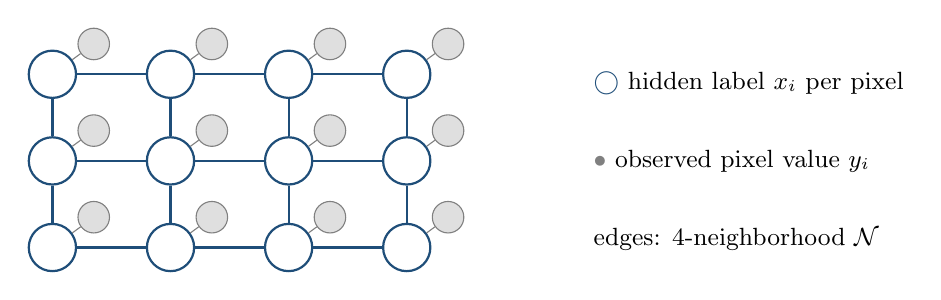
\begin{tikzpicture}[x=1.5cm, y=1.1cm,
  lab/.style={circle, draw=accent, thick, fill=white, minimum size=6mm, inner sep=0pt},
  obs/.style={circle, draw=gray, fill=gray!25, minimum size=4mm, inner sep=0pt}]
  \foreach \i in {0,1,2,3} \foreach \j in {0,1,2} {
    \node[obs] (y\i\j) at (\i+0.35,\j+0.35) {};
    \node[lab] (x\i\j) at (\i,\j) {};
    \draw[gray] (x\i\j) -- (y\i\j);
  }
  \foreach \i in {0,1,2} \foreach \j in {0,1,2} {
    \pgfmathtruncatemacro{\n}{\i+1}\draw[accent, thick] (x\i\j) -- (x\n\j);}
  \foreach \i in {0,1,2,3} \foreach \j in {0,1} {
    \pgfmathtruncatemacro{\n}{\j+1}\draw[accent, thick] (x\i\j) -- (x\i\n);}
  \node[anchor=west, font=\small, align=left] at (4.5,1.9)
    {\textcolor{accent}{$\bigcirc$} hidden label $x_i$ per pixel};
  \node[anchor=west, font=\small, align=left] at (4.5,1.0)
    {\textcolor{gray}{$\bullet$} observed pixel value $y_i$};
  \node[anchor=west, font=\small, align=left] at (4.5,0.1)
    {edges: 4-neighborhood $\mathcal{N}$};
\end{tikzpicture}
\end{center}
\noindent
A grid of hidden label variables $x_i$ (one per pixel), each connected to its
observation $y_i$ and to its 4 (or 8) neighbors. The energy is
\[
  E(\mathbf{x}) = \sum_i E_i(x_i, y_i) + \sum_{(i,j)\in\mathcal N} E_{ij}(x_i,x_j),
\]
\noindent
minimized (MAP labeling) with graph cuts, ICM, belief propagation, or
simulated annealing. Used for denoising, segmentation, stereo.

\q{103}{What does CRF stand for?}
\emph{Conditional Random Field}.

\q{104}{What is the basic difference between MRF and CRF?}
An MRF is \emph{generative}: it models the joint $p(\mathbf{x},\mathbf{y}) =
p(\mathbf{y}\mid\mathbf{x})\,p(\mathbf{x})$, the prior $p(\mathbf{x})$ on labels
is independent of the data, and the observations are assumed conditionally
independent given the labels. A CRF is \emph{discriminative}: it models the
posterior $p(\mathbf{x}\mid\mathbf{y})$ directly; all potentials, including the
pairwise ones, may depend on the entire observed image $\mathbf{y}$. Example:
a contrast-sensitive smoothness term that penalizes label changes less across
strong image edges.

% =====================================================================
\topic{Training Neural Networks}{Q105--Q111}

\idea{An MLP is a set of weights and biases; training moves them downhill on the
loss using gradients from backpropagation. Activation functions supply the
nonlinearity, and momentum and weight decay make the descent faster and the
result more general.}

\q{105}{What are the weights in an MLP?}
The learnable parameters on the connections: $w_{ji}$ scales the output $z_i$
of neuron $i$ before it enters neuron $j$. Their size and sign express how
strongly and in which direction an input influences a neuron. All knowledge of
the trained network is stored in weights and biases.

\q{106}{What is the bias term in an MLP?}
A constant $b_j$ added to the weighted sum, $a_j = \sum_i w_{ji}z_i + b_j$.
It shifts the activation threshold, i.e.\ moves the decision hyperplane away from
the origin. Implemented as the weight $w_{j0}$ of an additional input fixed to
$z_0 = 1$, and learned like any other weight.

\q{107}{What are common activation / transfer functions in an MLP?}
\begin{table}[ht]
  \centering\small
  \begin{tabular}{@{}lll@{}}
    \toprule
    Function & $f(a)$ & Derivative \\
    \midrule
    Step (Heaviside, perceptron) & $[a\ge 0]$ & $0$ a.e.\ (not usable for backprop) \\
    Logistic sigmoid & $\sigma(a) = 1/(1+e^{-a})$ & $\sigma(1-\sigma)$ \\
    Hyperbolic tangent & $\tanh(a)$ & $1-\tanh^2(a)$ \\
    ReLU & $\max(0,a)$ & $[a>0]$ \\
    Identity (regression output) & $a$ & $1$ \\
    Softmax (class output) & $e^{a_k}/\sum_l e^{a_l}$ & --- \\
    \bottomrule
  \end{tabular}
  \caption{Common activation functions.}
\end{table}

\q{108}{Which properties do transfer functions in an MLP usually have?}
Nonlinear (otherwise the stacked layers collapse into one linear map);
differentiable, at least almost everywhere (needed for backpropagation);
monotonically increasing; often bounded / saturating (sigmoid, tanh), which
squashes outputs into a fixed range; derivatives cheap to compute from the
function value itself.

\q{109}{What is the update rule for the weights in an MLP?}
Gradient descent with learning rate $\eta$:
\[
  w_{ji}^{(t+1)} = w_{ji}^{(t)} - \eta\,\frac{\partial E}{\partial w_{ji}}
  = w_{ji}^{(t)} - \eta\,\delta_j\, z_i ,
\]
\noindent
with $\delta_j$ from backpropagation (Q14) and $z_i$ the input on the
connection.

\q{110}{What is the difference between online, batch, and offline learning?}
They differ in how many training samples enter one weight update:
\begin{itemize}
  \item \emph{Online}: update after every single sample
    ($\Delta w = -\eta\,\partial e_n/\partial w$); many cheap, noisy steps.
  \item \emph{(Mini-)batch}: update after a small random subset of samples;
    the standard in practice (stochastic gradient descent).
  \item \emph{Offline} (full batch): sum the gradient over the whole training set,
    then update once per epoch; exact gradient but few, expensive updates.
\end{itemize}
\noindent
Note: in some texts ``batch'' means offline (full batch).

\q{111}{What is momentum / inertia and weight decay?}
\emph{Momentum}: add a fraction $\alpha$ of the previous update,
\[
  \Delta w^{(t)} = -\eta\,\frac{\partial E}{\partial w} + \alpha\,\Delta w^{(t-1)},
  \qquad 0\le\alpha<1 .
\]
\noindent
Like a heavy ball: consistent gradient directions accelerate, oscillations
cancel, flat regions and small local minima are passed.
\emph{Weight decay}: add the penalty $\tfrac{\lambda}{2}\|\mathbf{w}\|^2$ to the
loss, giving $w \leftarrow (1-\eta\lambda)\,w - \eta\,\partial E/\partial w$.
Weights shrink unless the data supports them; a regularizer against
overfitting.

% =====================================================================
\topic{Convolutional Networks}{Q112--Q117}

\idea{A ConvNet is an MLP adapted to images: neurons only see a local window
(receptive field) and share the same weights across positions, so a layer is a
convolution. Stacks of convolution, ReLU and pooling extract features; fully
connected layers classify. Dropout, data augmentation and pre-training fight
overfitting.}

\q{112}{What is meant by ``receptive field'' and ``shared weights'' in the
context of ConvNets?}
\emph{Receptive field}: the region of the input image that influences a given
neuron. Each neuron connects only to a small local neighborhood (e.g.\
$3\times3$) of the previous layer; through stacking, the receptive field grows
with depth. \emph{Shared weights}: all neurons of one feature map use the same
kernel weights at every position, so the layer computes a convolution. This
drastically reduces the number of parameters and makes the features
translation-equivariant (a pattern is detected wherever it appears).

\q{113}{Which activation function is usually used for ConvNets?}
ReLU, $f(a) = \max(0,a)$: cheap, does not saturate for positive inputs (less
vanishing gradient), sparse activations, faster training. Softmax at the output
for classification.

\q{114}{What is the basic architecture / layout of a ConvNet?}
\begin{center}
\resizebox{\linewidth}{!}{%
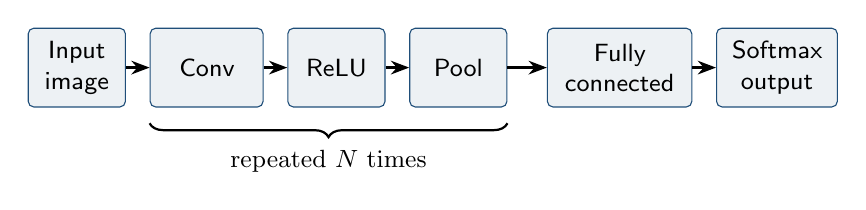
\begin{tikzpicture}[node distance=3mm,
  box/.style={draw=accent, fill=accent!8, rounded corners=2pt, align=center,
    font=\sffamily\small, minimum height=10mm},
  >={Stealth}]
  \node[box, text width=10mm] (i) {Input\\image};
  \node[box, right=of i, text width=12mm] (c) {Conv};
  \node[box, right=of c, text width=10mm] (r) {ReLU};
  \node[box, right=of r, text width=10mm] (p) {Pool};
  \node[box, right=5mm of p, text width=16mm] (f) {Fully\\connected};
  \node[box, right=of f, text width=13mm] (s) {Softmax\\output};
  \foreach \a/\b in {i/c,c/r,r/p,p/f,f/s} \draw[->, thick] (\a) -- (\b);
  \draw[decorate, decoration={brace, amplitude=5pt, mirror}, thick]
    ([yshift=-2mm]c.south west) -- ([yshift=-2mm]p.south east)
    node[midway, below=6pt, font=\small] {repeated $N$ times};
\end{tikzpicture}}
\end{center}
\noindent
Input $\rightarrow$ several blocks of [convolution $\rightarrow$ ReLU
$\rightarrow$ (max) pooling] $\rightarrow$ one or more fully connected layers
$\rightarrow$ softmax. Along the network the spatial resolution shrinks and
the number of channels (feature maps) grows; features become more abstract
(edges $\rightarrow$ textures $\rightarrow$ parts $\rightarrow$ objects).
Examples: LeNet, AlexNet, VGG.

\q{115}{What is dropout?}
A regularization technique: during training each neuron's output is set to
zero with probability $p$ (e.g.\ $0.5$), independently in every iteration.
Neurons cannot rely on specific other neurons (no co-adaptation), and training
effectively averages an ensemble of thinned networks. At test time all neurons
are used and activations scaled by $(1-p)$ (or, equivalently, activations are
scaled by $1/(1-p)$ during training).

\q{116}{What is meant with ``data augmentation''?}
Artificially enlarging the training set with label-preserving transformations
of the existing samples: flips, random crops and translations, rotations,
scaling, color and brightness jitter, noise. It reduces overfitting and teaches
invariance to these transformations.

\q{117}{How does pre-training a ConvNet work?}
Train the network first on a large dataset (e.g.\ ImageNet) for a generic task.
Then transfer it to the target task with little data: replace the output layer
to match the new classes, initialize the rest with the pre-trained weights, and
\emph{fine-tune} on the target data with a small learning rate. Alternatively
freeze the early layers (generic features such as edges and textures) and train
only the last layers, or use the network as a fixed feature extractor.
Historically, networks were also pre-trained unsupervised, layer by layer
(autoencoders, RBMs), before supervised fine-tuning.

\end{document}
